

\documentclass[preprint]{sigplanconf}
\usepackage[latin1]{inputenc}
\usepackage{times}
\usepackage{latexsym}
\usepackage{graphicx}
\usepackage{enumitem}
\usepackage{listings}
\usepackage{bussproofs}
\usepackage{comment}
\usepackage[numbers]{natbib}
\usepackage{graphicx} % Graphics support
\usepackage{caption} % Improved captions
\usepackage{subfig} % Inclusion of subfigures


\usepackage{tikz}
\usepackage{tikz-qtree}


% Set the overall layout of the tree
%\tikzstyle{level 1}=[level distance=3.5cm, sibling distance=3.5cm]
%\tikzstyle{level 2}=[level distance=3.5cm, sibling distance=2cm]

% Define styles for bags and leafs
%\tikzstyle{leaf} = [draw=none,fill=none, text width=4em, text centered]
%\tikzstyle{relation} = [ellipse, draw, text width=5em, text centered]
%\tikzstyle{branch} = [rectangle, draw, text width=6em, text centered]




%\usepackage{subfigure}

% adjust space between letters
\usepackage{microtype}

% adjust space between lines
\linespread{1.05}

% for header and footer
\usepackage{fancyhdr}

% change the font size of section
%\usepackage{sectsty}
%\sectionfont{\fontsize{12}{15}\selectfont}
%\subsectionfont{\fontsize{11}{14}\selectfont}

\lstset{morekeywords={in_range, in_rel, add, remove, Drop, Deliver, ForwardTo, Multicast, IpSrc, IpDst}}


\usepackage{amsmath, amssymb}

\pagestyle{fancy}

\lhead{Department of Computer Science\\
Princeton University}
\chead{}
% \rhead{\includegraphics[height=15mm]{princeton_logo.jpg}}
\lfoot{}
\cfoot{}
\rfoot{}

% remove page numbers
%\thispagestyle{empty}

% no indent at the start of paragraphs
\parindent=0em

% for increasing space between paragraphs
\newcommand{\emptyline}{\vspace{5pt}}

\title{Red Oak: Proactive Policy Generation}
 \authorinfo{Ryan Beckett}{Princeton University}{rbeckett@princeton.edu}
 \authorinfo{Olivier Savary B\'{e}langer}{Princeton University}{olivierb@princeton.edu}


%-----------------------------------------------------------

\begin{document}
\maketitle

\begin{abstract} ...
\end{abstract}

\section*{Introduction}

One of the major outcomes of the Software Defined Networking (SDN) movement has been a unified, open interface to the switch hardware. This has, in turn, enabled new opportunities for network programmability. The typical model for SDN involves a centralized controller or distributed set of controllers programming switches dynamically to implement the desired control functionality.
However, the questions remains as to how best to write programs for SDNs.

Recent collaborations between researchers in networking and programming languages have resulting in a number of new network-specific programming languages. One example is the Frenetic family of languages \cite{Frenetic}, which allow programmers to write simple packet processing functions in a domain-specific language and combine them together using policy combinators. Another approach, described in Maple \cite{Maple}, is to allow programmers to write policies in an arbitrary, high-level programming language as a function that takes a packet and produces a forwarding path, the algorithmic policy. Conceptually, the function is run anew on each packet that enters the network.

Ultimately, the performance requirements of networks dictate that the centralized controller(s) can not handle most traffic since redirecting packets to be handled by the controller incurs orders of magnitude increased latency compared to those being handled by switches. For this reason, compiler technologies for network programming languages must be able to push much of the control plane functionality into the data plane switches themselves. 

For Maple, the authors show how to optimize the controller so that packets are handled without having to run the function on them. Maple does so by providing a packet API capturing each access to packet fields, and memoizing the results of the function for subsequent packets sharing the accessed fields' values. Unfortunately, there are a number of limitations to this approach:


\begin{enumerate}
\item Since controller decisions are memoized, all initial packets must first go to the controller before it can learn how to forward similar packets directly in the data plane. This leads to a cold-startup phase with high packet latency.
\item The controller only observes concrete packets. This can lead to installing overly specialized forwarding rules on the switches that miss some of the high-level intent of the programmer (e.g., matching all packets with a particular IP prefix).
\item Most interesting network functions keep some global state (e.g., MAC learning table, ACLs). To ensure memoized decisions do not become invalid when the controller's environment (global state) changes, programmers must manually decide which previous decisions to invalidate.
\end{enumerate}


In this work, we language-independent API and compilation strategy that, like Maple, allows programmers to write network programs with the full generality of a high-level, general-purpose programming language.
However, we address each of the shortcomings in Maple listed above. Our contributions are the following:

\begin{enumerate}
\item We describe a static analysis on the user-defined forwarding policy that pushes symbolic packets through the function to explore all possible paths of execution. This analysis is then used to proactively generate forwarding rules to install in the network.
\item We provide a packet API that lets programmers ask if a field is in a particular range (e.g., IP prefix) rather than if the the field equals a particular value. This more expressive test works together with our analysis to better capture programmer intent when setting up forwarding decision in the data plane.
\item We provide a mutable relation data structure in our API to maintain global state. The data structure works together with our analysis to provide an automatic invalidation scheme. The analysis determines which future packets might affect global state and ensures that these relevant packets are actually seen by the controller.
\end{enumerate}



\section*{Algorithic Policies Revisited}
% Explains what algorithmic policies are, how maple was handling them and the difference with our model 
Algorithmic policies were introduced by Maple as a model for SDN controllers. An algorithmic policy is a programmer-defined function from a packet to a forwarding decision (i.e., where the packet(s) should end up). Conceptually this model offers the abstraction that the network forwards packets as if this function were executed on each packet when entering the network. To handle future traffic directly in the data plane, Maple keeps a tree data structure that branches on decisions observed at run time (e.g., the packet had source IP 10.0.0.1)


A policy for a simple stateful firewall using our API is included in Figure~\ref{fig:firewallcode}. For simplicity, we assume that IP ranges are between 0 and 1000, however it is easy to generalize this to actual IP prefixes.
In the example, source IPs from 0 to 10 are considered to be internal to the network and everything else, external. 

If a packet is sent from an internal host to an external host, the pair of internal and external host is added to a list of trusted connection. If a packet is received from an external host, we lookup in the table to see if the connection is trusted, in which case we forward the packet to its destination, otherwise we drop it. The forwarding decision "Deliver" is just shorthand for "forward the packet according to its intended destination".
An interesting point to be made about this function is that we are actively manipulating global policy state when we add entries to the stateful firewall's trusted connection relation.


\begin{figure}[ht]
\begin{lstlisting}
f(pkt):
  if in_range(pkt, src, 0, 10) then
     if in_range pkt dst  [(0,10)] then
        Deliver
     else 
        add pkt (IpDst, IpSrc) ``conn'';
        Deliver
  else if in_rel pkt (IpSrc,IpDst) ``conn'' then
         Deliver
       else
         Drop
       end
  end                
  \end{lstlisting}

\caption{A Stateful Firewall}
\label{fig:firewallcode}
\end{figure}

From an algorithmic policy such as the one included in Fig~\ref{fig:firewall-eg}, we generate a decision tree summarizing the function's interaction with the packet and the relevant decisions that will be made for particular classes of packets. The decision tree is created by analyzing the programmers function statically and then used by our runtime system to install switch rules and update them only when necessary (i.e., in response to changes in global state). For the stateful firewall included in figure~\ref{fig:firewallcode}, the following decision tree would be generated:


\begin{figure}[ht]
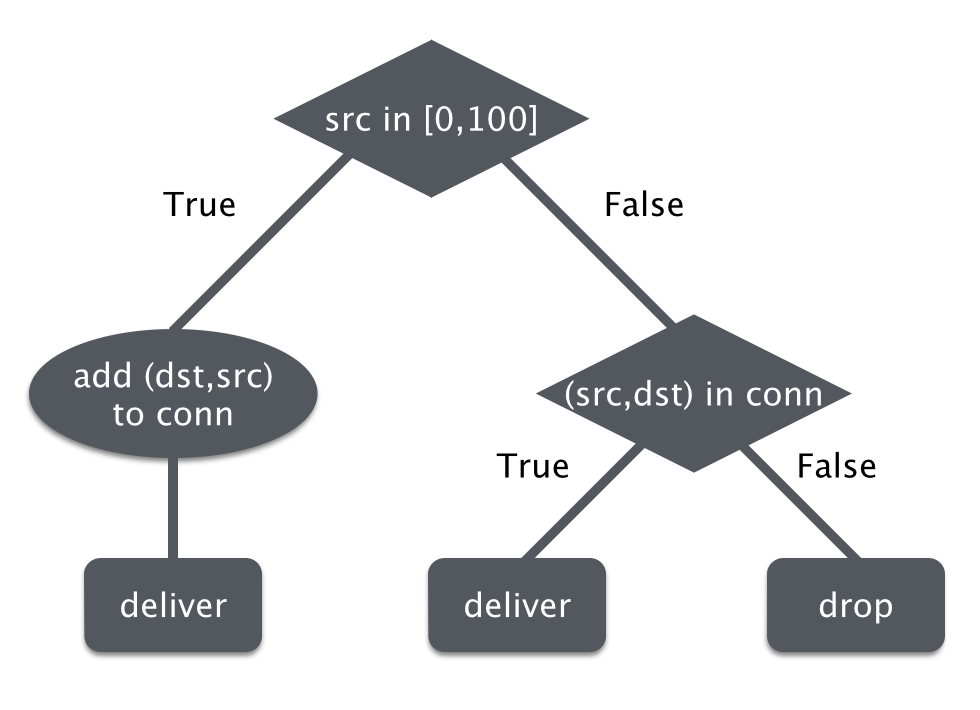
\includegraphics[scale=.5]{img/dtree.png}
\caption{Decision Tree for Stateful Firewall}     
\label{fig:decisiontree}  
  \end{figure}

This decision tree would, in turn, lead to the following set of prioritized symbolic rules. We call these symbolic rules because they represent constraints on the actual concrete rules. The concrete rules our system will install in the network depend on the current contents of the trusted connection relation. In particular, for each IP source that is trusted to communicate with an internal destination in the "conn" relation, we will get a concrete rule permitting this communication.
  \begin{lstlisting}
ipsrc in [0, 100] --> Sent to Controller
ipsrc in [101, 1000], (ipsrc,ipdst) in conn
                  --> Deliver
ipsrc in [101, 1000], (ipsrc,ipdst) not in conn
                  --> Drop
  \end{lstlisting}

After initialization (starting with no trusted connections), the concrete rules would be generated from the symbolic rules by having all relations be empty:
\begin{lstlisting}
ipsrc in [0, 100] ---> Sent to Controller  
ipsrc in [101, 1000] ---> Drop  
\end{lstlisting}
  

  When a packet is received, it is forwarded according to the first matching concrete rule installed on the switch. If the packet is sent to the controller, we evaluate the decision tree for that packet, potentially adding and removing tuples from relations, before forwarding the packet according to forwarding decision held in the relevant leaf of the decision tree. We then regenerate the concrete rules using the updated relation. 
  
 For example, after having seen a packet with \lstinline|ipsrc| 10 and \lstinline|ipdst| 150, the first rules would be matched, evaluating the decision tree would add tuple $(10,150)$ to relation \lstinline|conn|, the packet would be forwarded according to the forwarding decision \lstinline|Deliver|, and the concrete rules would updated as follow:

\begin{lstlisting}
ipsrc in [0, 100] ---> Sent to Controller  
ipsrc = 150, ipdst = 10 ---> Deliver  
ipsrc in [101, 1000] ---> Drop  
\end{lstlisting}
  
  

\section*{Algorithmic Policies and Decision Trees}
In this section, we describe how an algorithmic policy may interact with a packet and with relations to generate a forwarding decision, and how we build a decision tree out of an algorithmic policy.

   \subsection*{Range-based Branching}
   

   % Why range instead of actual value, pre-generation of rules using symbolic pre-execution
   Our API exports a single function for inspecting the contents of a packet's field, which is a test on the range of the packet's field. The ability to test if a value falls in a particular range is useful for capturing programmer intent with respect to things like IP prefix matching. Other tests on packet fields can be encoded in terms of ranges. For example, to test whether a field equals a particular value, one can simply test if it falls in the range with that value as both the lower and upper bound. Likewise, the programmer can test if a field is greater than or less than a particular value by testing if the field is in the range from the value to the maximum or minimum possible value for that field respectively. 
   
Conveniently, ranges on packet fields also give us a way to describe symbolic packets - packets that represent a set of concrete packets. Later we will see how our static analysis will proactively generate rules to install on the switch hardware by propagating symbolic packet ranges through the control structure of the program.

   % Can represent constraints on the ranges admissible given a certain topology as a series of ``true'' branches at the root of the tree.


     \subsection*{Built-in Relation with Automatic Invalidation}
   % Relation with add and remove tuple of fields from a relation (empty at the begining), Inhabitant-based Branching 
	Many network applications of interest need to keep around some global state to keep track of things that have happened in the network. A stateful firewall, like the one we introduced earlier, needs to maintain an ACL of external hosts that are trusted to communicate with internal hosts. This list can change over time as packets traverse the network. Likewise, a MAC learning application would need to remember where to send packets destined for particular Ethernet destinations. However, reasoning about which packets the controller needs to see, and how to set up forwarding rules in the data plane to ensure that these packets are actually seen by the controller is challenging for programmers.
	
	We introduce a simple table (relation) data structure that handles updating mutable, global state in the controller automatically. Intuitively, each time a table can be updated, the controller must witness the update. Our range-based analysis determines all possible packets that could reach code resulting in an update to the table and instruments the data plane with forwarding rules to send relevant traffic to the controller.

   
   % Computing which packets need to be sent to the controller (i.e. only the ones reaching an ``add'' or a ``remove'' node.

     
  

   \subsection*{Forwarding Decision}
   % can give constant decision (e.g. drop() or fwd(loc) to a certain location loc), or decision based on values of the packet (e.g. deliver() which forwards to dst)
	The programming model for Oak is that each packet entering the network is mapped to a forwarding decision that describes where the packet should end up leaving the network. For simplicity, we assume that we are targeting a one big switch implementation of the network. The one big switch model has been heavily optimized \cite{Obs}, and we view the problem of determining paths through the network as orthogonal to our work here. 
  
   We provide several types of forwarding decisions to the programmer. The programmer can deliver a packet, according to the packet's desination, drop a packet, and forwarding a packet to a static location. Our model also allows for dynamic forwarding based on component of relation, for example to the last seen location of a host according to a MAC-learning controller (not shown in Fig~\ref{fig:range_api}). Finally, the programmer can combine several forwarding decisions into one by using a mulitcast forwarding decision.
   

   \subsection*{Combining Algorithmic Policies}
   % cross, ``holes''
   As algorithmic policies under our model are functions of the host language, we inherit the latter's function space ability, allowing, amongst other things, for compositon of algorithmic policies and higher-order algorithmic policies.

\begin{figure}[ht]
\begin{lstlisting}

let filter_src_range f r pkt =
 if in_range pkt IpSrc r then
    f pkt
 else
   Drop   
\end{lstlisting}

\caption{Example of a Partial Algorithmic Policy}
\label{fig:ex-hole}
\end{figure}

   
   For example, we include in Figure~\ref{fig:ex-hole} the source code for \lstinline|filter_src_range| a partial policy, which, given a policy \lstinline|f| and a range \lstinline|r|, will forwards all packets whose source IP is within range \lstinline|r| and drop the packet otherwise. The ability to compose two or more policies in sequence like this arises many times in practice. In our earlier firewall example, instead of delivering packets that were not dropped, we could instead have deferred to another function to decide how to handle trusted traffic.


   \begin{figure}[ht]
\begin{lstlisting}
let f_cross (f_1) (f_2) pkt =
  let d_1 = f_1 pkt in
  let d_2 = f_2 pkt in
  Multicast (d_1,d_2)
\end{lstlisting}

\caption{Example of a Composition Operator}
\label{fig:ex-cross}
\end{figure}
   
Various composition operator may be built as host language function to combine multiple algorithmic policies into a single one. For example, \lstinline|f_cross|, included in Figure~\ref{fig:ex-cross}, runs algorithmic policy \lstinline|f_1| and \lstinline|f_2| on input packets and multicasts them according to both forwarding decisions. This corresponds to the parallel composition operator for the Frenetic language \cite{Frenetic}, however here the composition takes place in a fully general purpose language.
   
\section*{Implementation}
%that's the hope...

\subsection*{A.P.I.}
In our model, algorithmic policies interact with packets through A.P.I function calls before returning a forwarding decision. We include in Figure~\ref{fig:range_api} the core of our \lstinline|A.P.I.|. 
\lstinline|field| enumerates the different fields of a packet. It can be extended to represent more fields of a packet's header. Associated with \lstinline|field| are \lstinline|range|s, possible values taken by a certain packet's field, within a given minimum value \lstinline|min_value| and maximum value \lstinline|max_value|. \lstinline|range| consists of list of integer pairs, representing a collection of intervals whose union correspond to the range of values of a packet. For simplicity, we consider integer fields here, but this could be extended, for example, to IP prefix, boolean flags, etc.

\lstinline|forwarding_decision| enumerates the different forwarding decision which can be returned by an algorithmic policy. \lstinline|Deliver| forwards the packet to its destination, \lstinline|Drop| drops the packet, \lstinline|ForwardTo i| forwards the packet to a constant location \lstinline|i| and \lstinline|Multicast fd1 fd2| duplicates the packet and handles each according to \lstinline|fd1| and \lstinline|fd2| respectively.

Algorithmic policy may base their forwarding decision on the result of calling the \lstinline|in_range pkt fld r|, which returns whether value of packet \lstinline|pkt| at field \lstinline|fld| is in the range \lstinline|r|.

\begin{figure}[ht]
  \begin{lstlisting}
type packet

type field = IpSrc | IpDst 

type range = (int*int) list

val min_value: int 
val max_value: int

type forwarding_decision =
	| Deliver
	| Drop
	| ForwardTo of int
	| Multicast of forwarding_decision
                      * forwarding_decision


val in_range: packet -> field -> range -> bool
\end{lstlisting}

\caption{Signature of the packet and range-branching portion of the API}
\label{fig:range_api}
\end{figure}



In Figure~\ref{fig:rel_api}, we include the relation portion of the \lstinline|A.P.I.|, used to model stateful controller programs. A \lstinline|relation| represents a table in which each row contains a series of field values. It is referred to by a string. Policy writer may add a row to a relation \lstinline|rel| by calling the function \lstinline|add pkt flds rel|, which will populate the new row with the fields \lstinline|flds|' values of the current packet \lstinline|pkt|. Similarly, they may remove a row containing exactly the values of fields \lstinline|flds|' values of the current packet \lstinline|pkt| by calling \lstinline|remove pkt flds rel|. Finally, one may test if the values of fields \lstinline|flds| of current packet \lstinline|pkt| are in relation \lstinline|rel| by calling \lstinline|in_rel pkt flds rel|.



\begin{figure}[ht]
  \begin{lstlisting}
type relation = string

val add: packet -> field list -> relation -> unit

val remove: packet -> field list -> relation -> unit

val in_rel: packet -> field list -> relation-> bool
\end{lstlisting}

\caption{Signature of the relation portion of the API}
\label{fig:rel_api}
\end{figure}




\begin{figure}[ht]
  \begin{lstlisting}
val compile: (packet -> forwarding_decision)
    -> policy
    
val run: policy -> ((field * int) list) list
    -> unit
    
val print_policy: policy -> unit
  \end{lstlisting}

  \caption{Signature of the interactive portion of the API}
  \label{fig:build_api}
\end{figure}

\subsection*{Tracing the Algorithmic Policy}
From an algorithmic policy, we generate a decision tree  whose leaves are forwarding decision and whose node are either branching according the range of a field value, according to a relation ,or adding and removing components from a relation.

\begin{figure*}[ht]
\begin{lstlisting}
let compile (f: packet -> forwarding_decision) : policy =
      push most general packet to (empty) stack
      set the current location to be the root of an empty decision tree
      while (stack is not empty)
         pop the top of the stack as pkt
         run f of pkt resulting in a forwarding decision fd (and a modified packet pkt)
         record the forwarding decision for the symbolic packet pkt at the current location in the decision tree
         set the current location to be the root of the decision tree and repeat
  
\end{lstlisting}
\caption{Pseudocode for the compile function}
\label{fig:compile-pseudo}
\end{figure*}

To do so, we repeatedly run the algorithmic policy \lstinline|f| on symbol packets generated to explore every reachable path.
We begin by calling \lstinline|f| on a symbolic packet covering the full range of value for each of its fields.

When \lstinline|f| calls \lstinline|in_range| to learn if the field \lstinline|fld|'s value is in the range \lstinline|r|, we
\begin{enumerate}
\item  create an \lstinline|Inrange| branching node in the decision tree
\item refine the current symbolic packet to represent all packets in range \lstinline|r| that could reach this test in the algorithmic policy and return true
\item push on the stack of packets to process a symbolic packets representing all packets in the complement of \lstinline|r| for field \lstinline|fld|.
\end{enumerate}


Similarly, when the algorithmic policy calls \lstinline|in_relation| to learn if fields \lstinline|flds|'s value are in a relation \lstinline|rel|, we
\begin{enumerate}
  \item create an \lstinline|Inrelation| branching node in the decision tree
  \item tag the current packet as being in the relation, return true
  \item push on the stack of packets to process the same packet tagged as not being part of relation \lstinline|rel|.
\end{enumerate}
When \lstinline|f| calls \lstinline|add| or \lstinline|remove|, we record in the decision the current symbolic packet, the relation and the fields being added or removed from the relation before continuing with the execution of \lstinline|f|.


% Prune dead subtree on empty ranges and add/remove which do not affect any inhabitant-based branching.



When \lstinline|f| returns with a forwarding decision, we record it, paired with the current symbolic packet, as a leaf node at the current position in the decision tree. We then pop the next packet from the stack of packets to process and restart tracing the policy from the root of the decision tree, exploring another path of \lstinline|f|.  


\subsection*{Simulating the Network Controller}

We provide a function \lstinline|run| to simulate the controller policy on a sequence of packets. \lstinline|policy| is an abstract datatype solely returned by \lstinline|compile| (see Fig.~\ref{fig:compile-pseudo}). In addition to the policy, \lstinline|run| takes in a list of packets represented as list of pairs of \lstinline|field| and \lstinline|int|, representing the values of the different fields of the packet. We expect all fields to be set exactly once for each packet in the list.

\lstinline|run| starts by building the symbolic rules for the given policy, and generating the concrete rules assuming all relations to be empty. In sequence, packet are matched with the current concrete rules, recording the forwarding decision. If a packet is sent to the controller, we evaluate the policy on the packet, potentially adding or removing tuples from relations. We then re-generate the concrete rules with the updated relation, before recording the forwarding decision.

\begin{figure*}[ht]
\begin{lstlisting}
let run (pol: policy) (inputs: ((field*int) list) list) : unit =
      build the symbolic rules for policy pol
      generate the concrete rules with all relations empty
      for each packets in input,
          find the first of the current rule matching the packet, and record the forwarding decision fd
          if packet is sent to the controller then
              evaluate the policy on the packet, potentially adding or removing tuples from relations, record forwarding decision fd'
              regenerate concrete rules
              forward the packet according the forwarding decision fd'
          else
              forward the packet according to fd 
\end{lstlisting}

\caption{Pseudocode for the run function}
\label{fig:run-pseudo}
  \end{figure*}



\subsection*{Optimizations}
   % 1) expand tree before add/remove nodes with a match on that relation ( based on add(p); add(p) == add(p) so can shortcircuit if p is already in the relation)
The rules generated by the presented technique ensures that the only packets being forwarded to the controller are those reaching an add or a remove node and thus potentially modify the state of the controller. However, these packets do not always modify the state of the controller. For example, in the firewall example (see Fig~\ref{fig:firewallcode}), after seeing a first packet with an \lstinline|ipsrc| of 10 and \lstinline|ipdst| of 150, any subsequent packet with the same \lstinline|ipsrc| and \lstinline|ipdst| could be delivered without being first forwarded to the controller, as adding the same tuple to a relation is idempotent. By using both local and global transformations on the decision tree, we can get closer to an optimal amount of packet forwarded to the controller, where only packets modifying relations are seen by the controller.

We implemented in Red Oak, under \lstinline|o1|, a local transformation adding an \lstinline|in_rel| node before \lstinline|add| or \lstinline|remove| nodes. In the case of \lstinline|add|, the \lstinline|add| node is omited in the true branch of \lstinline|in_rel|, such that packets whose fields are already in the relation will not be seen by the controller due to this \lstinline|add| node. Similarly, we omit the \lstinline|remove| node in the false branch of \lstinline|in_rel|. In the firewall example (see Fig.~\ref{fig:firewallcode}), this would result the following decision tree:

\begin{figure}[ht]
  TODO
\caption{Optimized Decision Tree for Stateful Firewall}     
\label{fig:decisiontreeopt}  
  \end{figure}


From which the following symbolic rule would be generate:
\begin{lstlisting}
ipsrc in [0, 100], (ipdst, ipsrc) in conn
                  --> Deliver
ipsrc in [0, 100] --> Sent to Controller
ipsrc in [101, 1000], (ipsrc,ipdst) in conn
                  --> Deliver
ipsrc in [101, 1000], (ipsrc,ipdst) not in conn
                  --> Drop
\end{lstlisting}

With empty relation, the concrete rules would be the same as with the unoptimized decision tree. However, after seeing, for example, packet with \lstinline|ipsrc| 10 and \lstinline|ipdst| 150, the rules would be
\begin{lstlisting}
ipsrc = 10, ipdst = 150 ---> Deliver  
ipsrc in [0, 100] ---> Sent to Controller  
ipsrc = 150, ipdst = 10 ---> Deliver  
ipsrc in [101, 1000] ---> Drop  
\end{lstlisting}


Other optimizations may further reduce the number of packet sent to the controller. For example, we could remove \lstinline|add| node which are followed by \lstinline|remove| node for the same relation and tuple on all path without the change being observed by an \lstinline|in_rel| node. Similarly, we could detect and warn the user if an added tuple may never be observed by an \lstinline|in_rel| node, for example by switching \lstinline|ipsrc| and \lstinline|ipdst| in the add tuple of the stateful firewall example (see Figure~\ref{fig:firewallcode}). We leave the implementation of these optimizations as future work.


% probably no evaluation :(
\section*{Evaluation}
% 1) optimality w.r.t. packets seen by the controler?
% 2) more examples
% 3) simulated run


\section*{Related Work}
% deeper comparison with Maple

%???

\section*{Future Work and Conclusion}


\bibliographystyle{plainnat}
\bibliography{bibi}



\end{document}
